\section{Prototype Description}

The prototype is divided into 3 subsystems, which are the quadcopter, the ground station, and the vicon system, as seen in \figref{prototypediagram}. 

\begin{figure}[H] 
	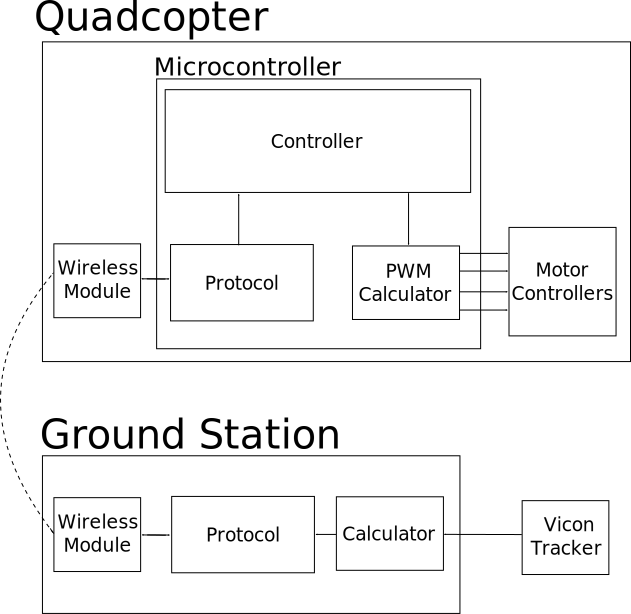
\includegraphics[scale=.5]{figures/prototypediagram}
	\centering
	\captionsetup{justification=centering}
	\captionof{figure}{Schematic diagram of the system, including the quadcopter, the ground station and the vicon system.}
	\label{prototypediagram}
\end{figure}

The quadcopter's most complex component is the microcontroller. It handles the control calculations, the PWM calculations according to the required control action and battery level, and the communication protocol necessary to exchange data with the ground station.

The microcontroller requires 4 PWM outputs with different and independent duty cycles for controlling the 4 motors in the quadcopter. 

The network interface in the microcontroller handles the incoming data from the ground station. This data consist of reference commands for the controllers and sensor data. It should also be able to send the battery voltage level to the ground station in order to detect when to end the flight.

The communication between the ground station and the quadcopter is done through wireless modules. These should allow the implementation of the communication by designing only the transport layer protocol.

The ground station gathers the information coming from the Vicon system and sends it to the quadcopter. This also includes doing calculations with the received Vicon data to obtain other variables like velocities or accelerations.

Finally, Vicon system uses the position of the markers placed in the quadcopter to provide its position and orientation. The orientation data is given in multiple forms but only Euler angles data is considered.

\textbf{Battery}

Voltage: 11.1 Volts

Discharge current: 20 Amperes

Weight: 141 grams

Capacity: 1500 mAh

\textbf{Propeller}



\textbf{Platform}

